\documentclass[border=10pt]{standalone}

\usepackage{tikz}
\usepackage{tikzsymbols}
\usetikzlibrary{calc,patterns,shapes.geometric}

\def\centerarc[#1](#2)(#3:#4:#5){\draw[#1] ($(#2)+({#5*cos(#3)},{#5*sin(#3)})$) arc (#3:#4:#5);}

\begin{document}
	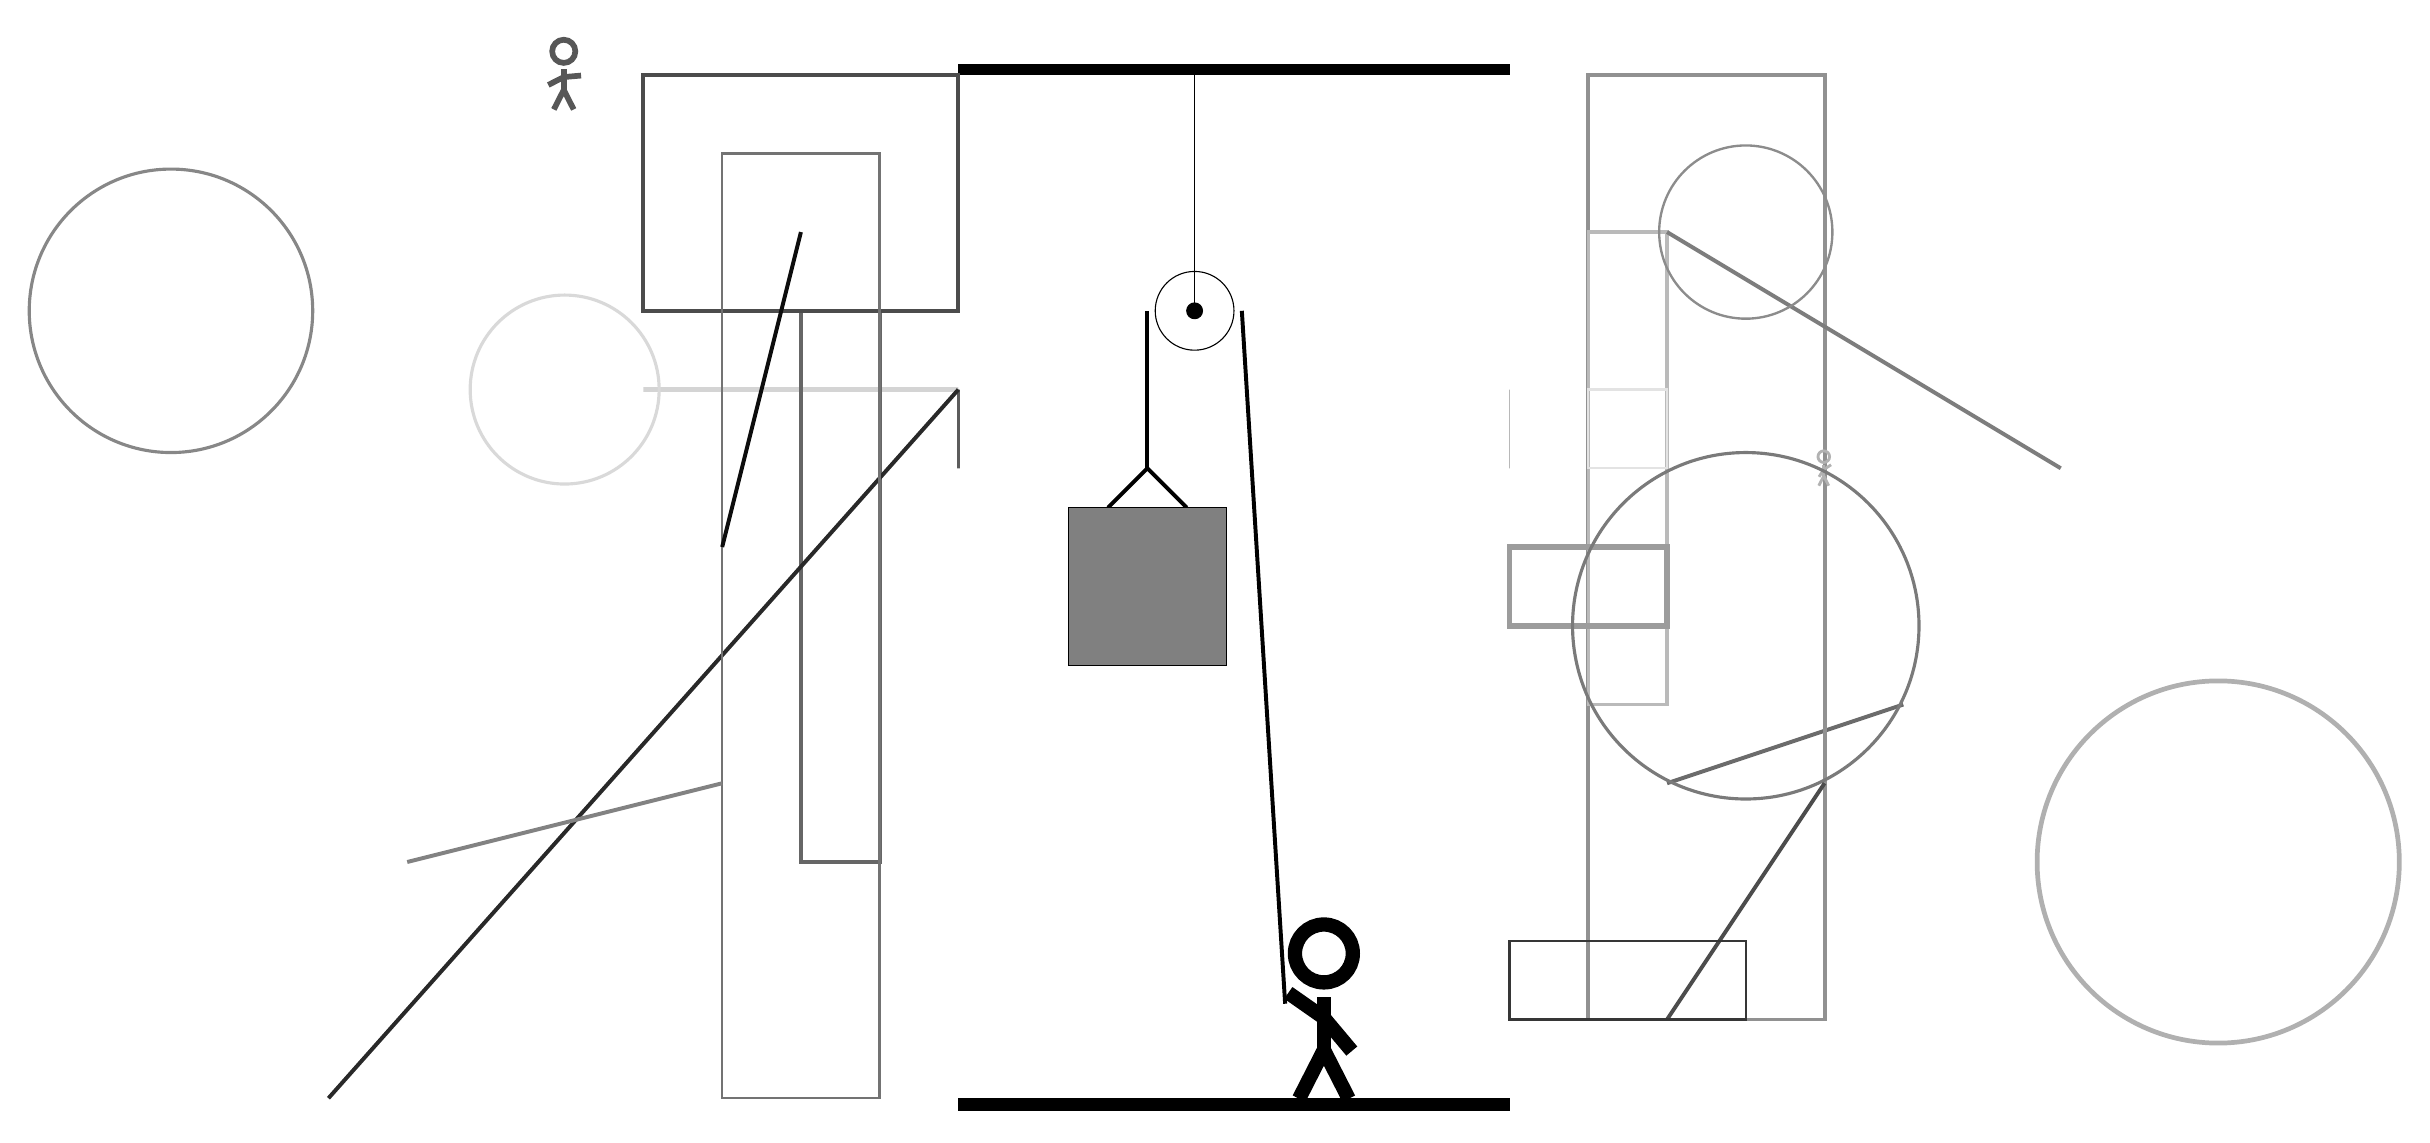
\begin{tikzpicture}
		%%%%% START %%%%%
		
		\draw[fill=black] (-2, 10) rectangle (5, 10.125);
		
		\draw (1, 7) circle (0.5);
		\draw[fill=black] (1, 7) circle (0.1);
		\draw (1, 10) -- (1, 7);
		
		\draw[line width=0.4mm, color=black!64] (-2, 6) rectangle (-2, 5);
		
		\draw[line width=0.5mm, color=black!58](7, 1) -- (10, 2);
		\draw[line width=0.5mm, color=black!43] (6, 10) rectangle (9, -2);
		\draw [line width=0.4mm, color=black!47](-12, 7) circle (1.8);
		\draw[line width=0.7mm, color=black!17] (-2, 6) rectangle (-6, 6);
		\draw[line width=0.5mm, color=black!60] (-4, 0) rectangle (-3, 7);
		\draw[line width=0.4mm, color=black!27] (7, 8) rectangle (6, 2);
		\draw[line width=0.2mm, color=black!28] (5, 6) rectangle (5, 5);
		\node[line width=0.5mm, color=black!30] at (9, 5) {\Strichmaxerl[2][57][33]};
		
		\draw[line width=0.5mm, color=black!51](7, 8) -- (12, 5);
		\node[line width=0.3mm, color=black!66] at (-7, 10) {\Strichmaxerl[4][27][5]};
		
		\draw[line width=0.5mm, color=black!70] (-2, 7) rectangle (-6, 10);
		\draw[line width=0.7mm, color=black!39] (7, 4) rectangle (5, 3);
		
		\draw[line width=0.5mm, color=black!84](-2, 6) -- (-10, -3);
		\draw[line width=0.3mm, color=black!55] (-3, -3) rectangle (-5, 9);
		\draw [line width=0.4mm, color=black!15](-7, 6) circle (1.2);
		
		\draw[line width=0.5mm, color=black!49](-5, 1) -- (-9, 0);
		\draw[line width=0.5mm, color=black!95](-5, 4) -- (-4, 8);
		\draw [line width=0.3mm, color=black!45](8, 8) circle (1.1);
		\draw[line width=0.3mm, color=black!11] (7, 6) rectangle (6, 5);
		\draw [line width=0.4mm, color=black!52](8, 3) circle (2.2);
		\draw[line width=0.5mm, color=black!70](9, 1) -- (7, -2);
		\draw[line width=0.3mm, color=black!79] (5, -2) rectangle (8, -1);
		\draw [line width=0.6mm, color=black!31](14, 0) circle (2.3);
		
		\draw[line width=0.5mm] (-0.1, 4.5) -- (0.4, 5.0) -- (0.9, 4.5);
		\draw[fill=black!50] (-0.6, 4.5) rectangle (1.4, 2.5);
		
		\draw[line width=0.5mm] (0.4, 7) -- (0.4, 5.0);
		\centerarc[line width=0.5mm](1, 7)(0:180:0.6);
		\draw[line width=0.5mm](1.6, 7) -- (2.15, -1.8);
		
		\node at (2.6, -1.9) {\Strichmaxerl[10][-35][-50]};
		
		\draw[fill=black] (-2, -3) rectangle (5, -3.15);
		
		%%%%% END %%%%%
	\end{tikzpicture}
\end{document}